\documentclass[
	12pt,                      % Schriftgroesse 12pt
	a4paper,                   % Layout fuer Din A4
	english,                   % neue deutsche Rechtschreibung nach der Reform
	oneside,                   % Layout fuer einseitigen Druck
	headinclude,               % Kopfzeile wird Seiten-Layouts mit beruecksichtigt
	headsepline,               % horizontale Linie unter Kolumnentitel
	plainheadsepline,          % horizontale Linie auch beim plain-Style
	BCOR=12mm,                  % Korrektur für die Bindung
	DIV=18,                    % DIV-Wert für die Erstellung des Satzspiegels, siehe scrguide
	parskip=half,              % Absatzabstand statt Absatzeinzug
	openany,                   % Kapitel können auf geraden und ungeraden Seiten beginnen
	bibliography=totoc,        % Literaturverz. wird in und sonstige verzeichnisse mit ins Inhaltsverzeichnis
	numbers=noenddot,          % Kapitelnummern immer ohne Punkt
	captions=tableheading,     % korrekte Abstaende bei TabellenUEBERschriften3
	]{scrbook}[2001/07/30]     % scrbook-Version mind. 2.8j von 2001/07/30

%##########################################################################################################
%
% Packete laden
%
%##########################################################################################################

\usepackage[english]{babel}
\usepackage[utf8]{inputenc}                    % Input-Encoding: ansinew for Windows
\usepackage[T1]{fontenc}                       % T1-kodierte Schriften, korrekte Trennmuster für Worte mit Umlauten
\usepackage{ae}                                % Für PDF-Erstellung

\usepackage[
	format=hang,
	font={footnotesize, sf},
	labelfont={bf},
	margin=1cm,
	aboveskip=5pt,
	belowskip=5pt,
	]{caption,subfig}                          % mehrzeilige Captions ausrichten; subfig: Untergrafiken
\usepackage{wrapfig}

\usepackage[centertags]{amsmath}               % AMS-Mathematik, centertags zentriert Nummer bei split
\usepackage{amssymb}                           % zusätzliche Symbole
\usepackage{trfsigns} 					       % für bestimmte Symbole
\usepackage{graphicx}                          % zum Einbinden von Grafiken
\usepackage[svgnames,table,hyperref]{xcolor}
\usepackage{float}                             % u.a. genaue Plazierung von Gleitobjekten mit H
\usepackage{epsfig}                            % eps Format für Grafiken
\usepackage[pdftex,pstarrows]{pict2e}
\usepackage{array}
\usepackage{listings}						   % Code-Einbindungsumgebung
\usepackage{courier}                           % verwende Courier statt cmtt als monospace-schrift
\usepackage{setspace}                          % Zeilenabstand einstellbar
\usepackage{rotating}
\onehalfspacing                                % eineinhalbzeilig einstellen
\usepackage{longtable}					       % Ermöglicht Tabellen die über den Seitenumbruch gehen (s. Symbolverzeichnis)
\usepackage{scrlayer-scrpage}
\usepackage{scrhack}                         % Kopf und Fusszeilen-Layout passt besser zur Dokumentklasse KOMA-Skript (scrbook) als das Pake fancyhdr, sonst ziemlich gleichwertig
\typearea[current]{current}                    % Neuberechnung des Satzspiegels mit alten Werten nach Änderung von Zeilenabstand,etc
\usepackage{xcolor,colortbl}                   % Packet um Tabellen bunt auszufüllen
\usepackage{wasysym}                           % Promillezeichen und co.
\usepackage{tabularx}
\usepackage{booktabs}
\usepackage{multirow}
\usepackage{braket}
\usepackage{algorithm}
\usepackage{algorithmic}
\usepackage{csquotes}
\usepackage{stix}           % changes all fonts !

% use Tikz to draw graphics
\usepackage{tikz}
\usetikzlibrary{shapes,arrows}
\tikzstyle{decision} = [diamond, draw, fill=red!20,
text width=4em, text badly centered, node distance=1.7cm, inner sep=2pt]
\tikzstyle{block} = [rectangle, draw, fill=blue!20,
text width=10em, text centered, rounded corners, node distance=1.35cm, minimum height=2em]
\tikzstyle{line} = [draw, -latex']
\tikzstyle{cloud} = [draw, circle, text centered, fill=red!20, node distance=4cm,
minimum height=1.5em, text width=2em]


\usepackage[
	backend=biber,
	style=chem-angew,			% Style Angewante Chemie
]{biblatex}     		 		% Biblatex Paket für Referenzen
\addbibresource{literatur.bib}	% File were you store sources

%##########################################################################################################
%
% PDF-Erzeugung: pdflatex statt latex aufrufen!
%
%##########################################################################################################

\pdfoutput=1
\usepackage[pdftex,  % muss letztes Package sein!
	pdftitle={Masterthesis},%
	pdfauthor={Andreas Hulm},%
	pdfsubject={free energy},%
	pdfkeywords={ ... },%
	pdfstartview={FitH},%
	pdfstartpage={5},%
	bookmarks,%
	raiselinks,%
	pageanchor,%
	hyperindex,%
	colorlinks,%
	citecolor=black!60!black,%
	linkcolor=black!70!black,%
	urlcolor=magenta!70!black,%
	filecolor=magenta!70!black,%
	menucolor=orange!70!black,%
    ]{hyperref}

%##########################################################################################################
%
% New- and Renew-Commands
%
%##########################################################################################################


\renewcommand{\headfont}{\normalfont\sffamily}             % Kolumnentitel serifenlos
\renewcommand{\pnumfont}{\normalfont\ttfamily\bfseries}    % Seitennummern typewriter und fett
\pagestyle{scrheadings}

% Einkommentieren falls beidseitige Darstellung erwünscht!!! aktuell definiert: oneside -> Layout fuer einseitigen Druck

%\ihead[]{\headmark}              % Kolumnentitel immer oben innen
%\ohead[\pagemark]{\pagemark}     % Seitennummern immer oben aussen
%\lefoot[]{}
%\rofoot[]{}                      % Seitennummern in der Fusszeile loeschen

\newcommand {\jkarray}[1]{\ensuremath{\underline{#1}}}
\newcommand {\jkmatrix}[1]{\ensuremath{\underline{\underline{#1}}}}
\newcommand {\einheit}[1]{\ensuremath{\mathrm{\left[#1\right]}}}
\newcommand {\lived}[2]{($\ast$#1, $\dagger$#2)}  %



%###########################################################################################################
%
% Parameter für die jeweiligen Packete definieren
%
%###########################################################################################################

\lstdefinestyle{cppcode}{language={[Visual]C++},%
	basicstyle=\ttfamily\footnotesize,%
	keywordstyle={\color{Navy} \bfseries},%
	identifierstyle={\color{DarkRed}},%
	commentstyle={\color{DarkOrange!50!black}\slshape},%
	stringstyle={\color{DarkGreen}},%
	showstringspaces=false,%
	backgroundcolor={\color{LightSkyBlue!40}},%
	columns=fixed,%
	keepspaces=true,%
	basewidth={0.55em},%
	frame=shadowbox,%
	rulesepcolor=\color{Gray},%
	breaklines=true,%
	numbers=left,%
	numberstyle=\tiny,%
	escapeinside={°(}{)°},%
	moredelim={[is][\bfseries]{°^}{^°}},%
	belowcaptionskip=0.5cm%
	}%

\lstdefinestyle{fort}{language={[95]Fortran},%
	basicstyle=\ttfamily\small,%
	keywordstyle={\color{Navy} \bfseries},%
	identifierstyle={\color{DarkRed}},%
	commentstyle={\color{DarkOrange!50!black}\slshape},%
	stringstyle={\color{DarkGreen}},%
	showstringspaces=false,%
	backgroundcolor={\color{LightSkyBlue!40}},%
	columns=fullflexible,%
	keepspaces=true,%
	basewidth={0.6em},%
	rulesepcolor=\color{Gray},%
	frame=shadowbox,%
	escapeinside={°(}{)°},%
	moredelim={[is][\bfseries]{°^}{^°}},%
	belowcaptionskip=0.5cm%
	}%


\lstdefinestyle{pseudocode}{basicstyle=\ttfamily\small,%
	columns=fixed,%
	keepspaces=true,%
	basewidth={0.55em},%
	frame=shadowbox,%
	backgroundcolor={\color{LightSkyBlue!40}},%
	rulesepcolor=\color{Gray},%
	escapeinside={°(}{)°},%
	moredelim={[is][\bfseries]{°^}{^°}},%
	belowcaptionskip=0.5cm%
	}%

\lstdefinestyle{maple}{%
	basicstyle=\sffamily\small\color{Red}\bfseries,%
	rulecolor=\color{Black},%
	columns=fixed,%
	keepspaces=true,%
	basewidth={0.55em},%
	frame=shadowbox,%
	numbers=left,%
	numberstyle=\tiny\color{Black},%
	numberblanklines=false,%
	rulesepcolor=\color{Gray},%
	breaklines=true,%
	breakautoindent=true,%
	backgroundcolor={\color{LightBlue!60}},%
	rulesepcolor=\color{Gray},%
	escapeinside={°(}{)°},%
	moredelim={[is][\bfseries]{°^}{^°}},%
	belowcaptionskip=0.5cm%
	}%

\lstdefinestyle{matlab}{language={Matlab},%
	basicstyle=\ttfamily\small,%
	keywordstyle={\color{Navy} \bfseries},%
	identifierstyle={\color{DarkRed}},%
	commentstyle={\color{DarkOrange!50!black}\slshape},%
	stringstyle={\color{DarkGreen}},%
	showstringspaces=false,%
	backgroundcolor={\color{LightSkyBlue!30}},%
	breaklines=true,%
	breakautoindent=true,%
	columns=fullflexible,%
	keepspaces=true,%
	basewidth={0.6em},%
	rulesepcolor=\color{Gray},%
	frame=shadowbox,%
	numbers=left,%
	numberstyle=\tiny\color{Black},%
	escapeinside={°(}{)°},%
	moredelim={[is][\bfseries]{°^}{^°}},%
	belowcaptionskip=0.5cm%
	}%

\lstdefinelanguage{Python}{
	basicstyle=\ttfamily\small,%
	keywordstyle={\color{Navy} \bfseries},%
 	keywords={typeof, null, catch, switch, in, int, str, float, self, boolean, throw, import,return, class, if ,elif, endif, while, do, else, True, False , catch, def, from, for},
 	identifierstyle=\color{black},
	comment=[l]{\#},
	commentstyle={\color{gray}\slshape},%
	stringstyle={\color{DarkGreen}},%
	backgroundcolor={\color{LightSkyBlue!30}},%
	breaklines=true,%
	breakautoindent=true,%
	columns=fullflexible,%
	keepspaces=true,%
	basewidth={0.6em},%
	rulesepcolor=\color{Gray},%
	frame=shadowbox,%
	numbers=left,%
	numberstyle=\tiny\color{Black},%
	escapeinside={°(}{)°},%
	moredelim={[is][\bfseries]{°^}{^°}},%
 	sensitive=false,
 	morecomment=[s]{/*}{*/},
	belowcaptionskip=0.5cm%
}

\graphicspath{{figs/}{bilder/}{plots/}}    % Falls texinput nicht gesetzt -> Bildverzeichnisse

% hier sind Worte zu definieren die in der Worttrennung falsch oder nicht erkannt werden!

\hyphenation{Post-pro-cess-ing--In-te-gral}


%###########################################################################################################
%
% Aufbau des Dokuments -> Einfügen der einzelnen Teile
%
%###########################################################################################################

% '''''''''''''''''''''''''''''''''''''''''''''''''''''''''''''''''''''
\newcommand{\sectionnumbering}[1]{%
	\setcounter{section}{0}%
	\renewcommand{\thesection}{\csname #1\endcsname{section}}}
% '''''''''''''''''''''''''''''''''''''''''''''''''''''''''''''''''''''

\newcounter{romanPagenumber} % neuen Seitenzähler als Variable definieren

\begin{document}
	\frontmatter

	\setheadsepline{0.0pt} 		  %Dicke der Trennlinie Kopfzeile - Text -> für Erklärung Änderungen ausschalten und erst ab Kurzzusammenfassung beginnen!

	\pagenumbering{Roman}         % romanische Nummerierung für die Deckblätter, Inhaltsverzeichnis und co.

	%
\begin{titlepage}

\begin{center}
{
%\fontsize{18}{18}\selectfont   % font Gr��e undefiniert-> es wird nur mit \text gearbeitet

\vspace*{-1.5cm}
\hfill \includegraphics*[width=3cm, keepaspectratio=true]{lmulogo.png}

\hrule                                 % horizontale Linie ein

\textsc{\LARGE Ludwig-Maximilians-University Munich}\\[2cm]

\textsc{\Large }\\[0.5cm]

\textsc{\Large Faculty of Chemistry and Pharmacy}\\[2.5cm]

\textbf{\LARGE Advanced enhanced sampling algorithms for free Energy calculation in collective variable space} \\[0.5cm]

\textsc{\Large Master Thesis in Theoretical Chemistry}\\[2.0cm]

\textsc{AK Ochsenfeld}\\[2.0cm]

\textsc{by}\\
\textsc{Andreas Valentin Hulm} \\[1,5cm]
%\textsc{geboren am 29.04.1997} \\
%\textsc{in Freising} \\ [2,5cm]

%Beginn der Bachelorarbeit: 07.05.2018 \\
%Bachelorarbeit beim Pr�fungsamt eingereicht am \today

\vspace{3.5cm}


}
\end{center}

\end{titlepage}


%\thispagestyle{empty}     % 2. Seite leer!
%\section*{}
     % Deckblatt Titel
	%
\begin{titlepage}

\begin{center}

{\fontsize{14pt}{14}

\textsc{Master Thesis in Theoretical Chemistry} \\
\vspace{0.5cm}
\textsc{submitted to the LMU Munic}\\
\vspace{0.5cm}
\textsc{at the Department of Chemistry}\\
\vspace{0.5cm}
\textsc{}\\[3cm]

\textsc{\Large  \underline{Subject:}}\\[3.0cm]

\textbf{\Large Advanced enhanced sampling algorithms for free Energy calculation in collective variable space}\\[6cm]
}
{\fontsize{12pt}{12} \selectfont%
\begin{tabular}{ll}
Verfasser:& Andreas Valentin Hulm \\
Matrikelnummer:& 11353987\\
Referent:& Prof. Dr. Christian Ochsenfeld\\
Betreuer:& Dr. Johannes Dietschreid\\[1cm]
Begonnen am:& October 02, 2020\\
Eingereicht:& \today\\
Abschließend beurteilt am:&   \hspace{4cm} Note: \\
\end{tabular}
}
\end{center}

\end{titlepage}

	\addchap{List of symbols}
\markboth{List of symbols}{List of symbols}
\label{cha:symbols}

\begin{longtable}[l]{lcp{10cm}}
	ABF		&&  Adaptive-biasing Force \\
	eABF  &&  extended Adaptive-biasing Force \\
  US    &&  Umbrella sampling \\
	WTM   &&  Well-Tempered Metadynamics \\
\end{longtable}


	\setheadsepline{0.5pt}        % Dicke der Trennlinie Kopfzeile - Text

	\tableofcontents              % Inhaltsverzeichnis

	\clearpage

	\setcounter{romanPagenumber}{\value{page}} % eigener Seitenzähler erhält aktuelle römische Seitenzahl

	\mainmatter                   % den Hauptteil beginnen
	\pagenumbering{arabic}        % ab hier wieder arabische Nummerierung

	\chapter{Introduction}
\label{cha:introduction}
Free energy differences are the driving force of chemical processes at or near thermodynamic equilibrium and therefore the central quantity that determines the behavior of these systems.\autocite{chipot2007free}
However, the calculation of free energies still constitutes one of the major challenges of computational chemistry.\autocite{kastner2011umbrella}
This is because free energy contains entropy, which is a measure for the available space of a system.
For more than a few atoms, mapping available space requires extensive sampling, making free energy calculations computationally exceedingly demanding.\autocite{kollman1993free}
Therefore, although the statistical-mechanical foundations for the calculation of free energy curves were laid decades ago,\autocite{chipot2007free} it is only in recent years that increasing computational power combined with major advances in the efficiency of quantum-mechanical/molecular-mechanical (QM/MM) codes\autocite{ochsenfeld2007linear,shao2015advances,acun2018scalable} made their application possible.
Today free energy calculations are frequently used in several important areas ranging from biochemistry\autocite{gumbart2013standard,fu2017new,capelli2019chasing}, to pharmacology\autocite{yu2017computer,sinko2013accounting} or
nanotechnology.\autocite{fu2017lubricating,chen2019tumbling}

In practice to sample configurations of chemical systems time trajectories are calculated by means of molecular dynamics (MD) or Monte-Carlo (MC) simulations.\autocite{ponder2003force,burke2012perspective}
However, as most chemical reactions involve crossing of free energy barriers, reaction coordinates often constitute slow degrees of freedom.
This means that trajectories stay kinetically trapped in \textit{metastable} states, e.g., the educt or product state, and are unable to explore the full reaction coordinate.\autocite{chipot2007free}
%Simple trajectories are therefore poorly suited for sampling of reaction coordinates.\autocite{chipot2007free}
To address this problem the vary active research field of \textit{enhanced sampling} emerged, which has already produced numerous different approaches to speed up exploration of reaction coordinates.
\autocite{jiang2010free, sugita1999replica,den2000thermodynamic, ciccotti2005blue, barducci2008well}

One particular successful class of algorithms relies on the definition of \textit{collective variables} (CVs).
This variables need to distinguish between the educt and product states, while ideally capturing all slow degrees of freedom along the way.\autocite{fiorin2013using}
Typically maximal two dimensional variables are chosen, because of the massive growth of computational cost of sampling in higher dimensional space, also known as \textit{curse of dimensionality}.\autocite{koppen2000curse}
The potential energy or forces along the CVs are then altered in a way, that increases the time spent in important regions.
One of the oldest and most widespread approaches is \textit{Umbrella Sampling}\autocite{kastner2011umbrella}, where bias potentials along the reaction coordinate drive a system from the reactant to the product state.
The intermediate steps are covered by a series of windows, in each of which a MD simulation is performed.
From this simulations the full free energy curve can be calculated by combining all windows with the weighted histogram analysis method (WHAM).\autocite{kumar1992weighted}
This approach enables efficient sampling along the reaction coordinate due to parallelisation.
However, it also requires some knowledge of the free energy curve prior to simulation in order to adequately choose the bias potentials.
In addition, setting up and analyzing multiple MD simulations requires huge computer resources and is time consuming.

To address both shortcomings this thesis will focus on another class of enhanced sampling algorithms, termed \textit{adaptive biasing} methods.\autocite{barducci2008well,comer2015adaptive,lesage2017smoothed}
Here a time-dependent, self-learning bias potential or force is introduced, that evolves during the simulation to encourage uniform sampling along the CV.
One can think of two complementary approaches to build time-dependent biases:
The first one, e.g., \textit{metadynamics} (MtD)\autocite{barducci2011metadynamics} and its variants, encourages sampling by flooding valleys of the free energy landscape with a time-dependent potential.
Because of its simplicity and straightforward implementation it has been integrated in almost all popular MD engines and was broadly utilized for a large variety of problems.\autocite{vymetal2011gyration,tanida2020alchemical,ikeda2005hydration}
The second one, termed \textit{adaptive biasing force} (ABF)\autocite{comer2015adaptive} method, flattens the free energy landscape by application of a time-dependent bias force.
Despite its outstanding stability and beneficial formal convergence properties, the practical implementation and application of ABF has been thwarted by the analytical formulation of the biasing forces, thereby limiting the scope of the numerical scheme.\autocite{fiorin2013using}
Recently this limitations could been lifted by extended-Lagrangian based methods, where a fictitious particle is coupled to the CV.
In this framework the bias force used for enhanced sampling only acts on the fictitious particle, which renders its implementation trivial.
The resulting extended-system ABF (eABF)\autocite{lesage2017smoothed} method combines the wide applicability of MtD with the convergence properties of ABF.
Additionally the calculation of free energy curves can be separated from sampling acceleration with an asymptotically unbiased free energy gradient estimator, termed \textit{corrected z-averaged restraint} (CZAR).\autocite{lesage2017smoothed}
The resulting flexibility in the choice of bias force can be used to combine both metadynamics and ABF to well-tempered metadynamics extended-system ABF (WTM-eABF),\autocite{fu2018zooming,fu2019taming} a highly potent enhanced-sampling scheme, which stands out due to its efficiency and robustness.

In this thesis all aforementioned adaptive biasing algorithms are combined with highly efficient QM/MM calculations in the in-house FermiONs++\autocite{kussmann2013linear} program package, to enable the broad application of free energy calculations for large molecular systems at accurate level of theory.

	\chapter{Theoretical Background}
\label{cha:theory}

\section{Statistical thermodynamics and free energy differences}

The formulation of the problem of free energy estimation starts with the Hamiltonian
\begin{equation}
  \textbf{H}(\textbf{r})=\sum_{i=1}^{N}\frac{\textbf{p}_{i}^2}{2m_i} + U(\textbf{x}_1,...,\textbf{x}_N)
\end{equation}
of an arbitrary chemical system, where $\textbf{r}=(\textbf{x}_1,...,\textbf{x}_N,\textbf{p}_1,...,\textbf{p}_N)$ denotes a point in the phase space of the N-particle system of interest and $U(\textbf{x}_1,...,\textbf{x}_N)$ is the potential energy of the system given by any quantum chemical method or force field. If the canonical ensemble (an ensemble with fixed number of particles N, volume V and temperature T) of such a system is sampled, for example by means of Langevin dynamics with sufficiently soft damping and small stochastic forces, the probability distribution $\rho(\textbf{x})$ in the configuration space $\textbf{x}$ follows the Boltzmann distribution
\begin{equation}
  \rho(\textbf{x})=\frac{e^{-\beta U(\textbf{x})}}{\int e^{-\beta U(\textbf{x})} d\textbf{x}}=Q^{-1}e^{-\beta U(\textbf{x})}
\end{equation}
were $Q$ denotes the partition function and $\beta=(k_B T)^{-1}$ the inverse temperature, $k_B$ is the Boltzmann constant. The partition function is the central quantity of statistical thermodynamics, relating macroscopic thermodynamic quantities to the microscopic details of a system. The free energy difference between two states A and B is defined by the ratio of the corresponding partition functions $Q_A$ and $Q_B$.
\begin{equation}
  A = -\beta^{-1}\ln \frac{Q_A}{Q_B}
\end{equation}
This immediately shows that the challenge of calculating free energies really consists in exploring the configuration space of a system such that relevant states are adequately sampled.



\section{Adaptive Biasing Methods}
\label{sec:adaptive biasing}

Instead of dividing the reaction coordinate in several windows, with adaptive biasing methods the free energy can be estimated from one single simulation. For this purpose the systems dynamics are biased towards states corresponding to large values of the free energy along the transition coordinate via a history-dependent biasing potential. In contrast to other importance sampling strategies like umbrella sampling, this methods require no prior knowledge of the free-energy landscape at hand. Instead, the biasing potential automatically converges towards the free energy, enabling diffusive behavior along the transition coordinate.

There are multiple adaptive biasing methods available, only differing in the choice of bias. Methods based on metadynamics (metaD) disfavor already visited states by accumulating repulsive potentials along the reaction coordinate (section \ref{sec:metaD}), while adaptive biasing force (ABF) methods compensate the mean force along the reaction coordinate to obtain uniform sampling (sections \ref{sec:ABF} and \ref{sec:eABF}). Meta-eABF combines both complementary approaches to speed up the convergence of the free energy estimate (section \ref{sec:meta-eABF}).

In principle adaptive biasing methods only rely on the sampling of the canonical ensemble. One simple way to achieve this is using Langevin dynamics with sufficiently soft damping and small stochastic forces. A schematic procedure of adaptively biased Langevin dynamics is given in Algorithm \ref{alg:ABM}.

\begin{algorithm}[H]
  \caption{Velocity Verlet integrator for adaptively biased Langevin dynamics with atomic masses $\textbf{M}$, coordinates $\textbf{x}(t)$, momenta $\textbf{p}(t)$, potential $V(\textbf{x}(t))$, forces $F(\textbf{x}(t))$ and friction coefficient $\gamma$,}
  \label{alg:ABM}
    \begin{algorithmic}
      \WHILE{$t < t_{end}$}
        \STATE
            \STATE $\textbf{p}(t+\frac{1}{2}\Delta t) \leftarrow \textbf{p}(t) + \frac{1}{2} \bigl(F(\textbf{x}(t))dt-\gamma \textbf{M}^{-1}\textbf{p}(t) dt + \sqrt{2\gamma\beta^{-1}}dW_t \bigr)$
        \STATE /* Get momenta at half time step
        \STATE
            \STATE $\textbf{x}(t+\Delta t) \leftarrow \textbf{x}(t) + \frac{2}{2+\gamma dt}\textbf{M}^{-1} \textbf{p}(t+\frac{1}{2}\Delta t) dt$
        \STATE /* Propagate coordinates
        \STATE
        \STATE $F(\textbf{x},t+\Delta t) \leftarrow - \nabla V(\textbf{x}(t+\Delta t))$
        \STATE /* get QM or MM forces $F(\textbf{x}(t))$ for new coordinates
        \STATE
        \STATE $F(\textbf{x},t+\Delta t) \leftarrow F(\textbf{x},t+\Delta t) + F^{bias}(\textbf{x},t+\Delta t)$
        \STATE /* call adaptive biasing routine to update bias force
        \STATE
            \STATE $\textbf{p}(t+\Delta t) = \frac{2 - \gamma dt}{2+\gamma dt} \textbf{p}(t+\frac{1}{2}\Delta t) - \frac{1}{2} \bigl(F(\textbf{x}(t+\Delta t))dt-\gamma \textbf{M}^{-1}\textbf{p}(t+\frac{1}{2}\Delta t)) dt + \sqrt{2\gamma\beta^{-1}}dW\bigr)$
        \STATE /* Get momenta at full time step
        \STATE
      \ENDWHILE
    \end{algorithmic}
\end{algorithm}

\subsection{Well-Tempered Metadynamics (WT-MetaD)}
\label{sec:metaD}

MetaD biases a systems dynamic towards undersampled regions along the reaction coordinate $\xi(\textbf{x})$, by accumulating repulsive potentials in regions that have already been visited. The bias potential is typically build by a superposition of repulsive Gaussian kernels and can be written:\autocite{barducci2011metadynamics}
\begin{equation}
  V^{metaD}(\xi,t)= \sum_{k<\frac{t}{\tau_G}} \tau_G \omega \exp\biggr(-\sum_{i=1}^{N_{dim}} \frac{1}{2\sigma_{i}^{2}} (\xi_{i}(\textbf{x})-\xi_{i}(\textbf{x},t_k))^2 \biggl)
\end{equation}
with deposition rate $\tau_G$, Gaussian height $\omega=W/\tau_G$ and variance $\sigma^2$ as free input parameters. In practice $V^{metaD}(\xi,t)$ is stored on a grid and updated every $\tau_G$ time steps for computational efficiency. Over the course of a simulation the bias potential fills local minima along the reaction coordinate until the systems evolution finally resembles a Brownian motion along the flattened free energy surface. The converged bias potential provides an unbiased estimate of the underlying free energy surface
\begin{equation}
  V^{metaD}(\xi, t \to \infty) = - A(\xi) + C
\end{equation}
To avoid oscillation of $V^{metaD}$ around the correct free energy, Well-Tempered metadynamics (WTM) introduces an additional scaling factor of the Gaussian height:\autocite{barducci2008well}
\begin{equation}
  \omega(\xi,t) = \frac{W}{\tau_G}\exp\biggl(-\frac{V^{WTM}(\xi,t)}{k_B \Delta T} \biggr)
\end{equation}
ensuring an decrease of $\omega$ over time and smooth convergence of the Well-Tempered bias potential $V^{WTM}(\xi,t)$. However, the new bias potential does not fully compensate the free energy surface, but can be controlled by parameter $\Delta T$. For $T \to 0$ the bias is zero and ordinary MD is recovered, whereas the limit $\Delta T \to \infty$ corresponds to normal metaD. To obtain a unbiased free energy estimate from $V^{WTM}(\xi,t)$ it has to be scaled accordingly:
\begin{equation}
A(\xi) = -\frac{T+\Delta T}{\Delta T}V^{WTM}(\xi, t)
\end{equation}

\subsection{Adaptive Biasing Force Method (ABF)}
\label{sec:ABF}

The intuition behind ABF is, that adding a force $A'(\xi(\textbf{x}))\nabla \xi(\textbf{x})$ that exactly compensates the average of the original force $-\nabla V(\textbf{x})$ along a given coordinate would result in uniform sampling along this coordinate.\autocite{comer2015adaptive}
Historically, this idea emerged from thermodynamic integration (TI), were the free energy derivative  is computed as the ensemble average of the instantaneous force, $F$, acting along a given reaction coordinate $\xi: \mathbb{R} ^{3N} \to \mathbb{R}$:
\begin{equation}
\frac{dA}{d\xi} = -\braket{F}_{\xi}
\end{equation}
and the free energy is calculated as the integral over this force.\autocite{kirkwood1935statistical,zwanzig1954high}
In practice, as one has no prior knowledge of the free energy derivative, ABF uses an on-the-fly estimate of the mean force acting along the reaction coordinate. For this purpose the transition coordinate $\xi$, connecting two end points, is divided in $M$ equally spaced bins. The approximation of the bias force $\overline{F}(N_{Step},k)$ in bin $k$ is than the average of all collected force samples:\autocite{comer2015adaptive}
\begin{equation}
  \overline{F}(N_{Step},k) = \frac{R(N_{Step}^k,k)}{N_{Step}^{k}} \sum_{\mu=1}^{N_{Step}^{k}} F_{\mu}^{k}
  \label{eq:mean force}
\end{equation}
\begin{equation}
  R(N_{step}^k,k)=\left\{\begin{array}{ll} N_{full}, & N_{step}^{k} < N_{full} \\
                                         1,  & N_{step}^{k} \geq  N_{full} \end{array}\right. \label{eq:ramp}
\end{equation}
with the linear ramp function $R(N_{step}^k,k)$ preventing large fluctuations of the force estimate at the beginning of the simulation from driving the system away from equilibrium. The number of samples when the full biasing force is applied, $N_{full}$, and the bin size are the only free parameters that have to be chosen by the user before the simulation. For a sufficiently large number of samples $N_{step}^k$ equation \ref{eq:mean force} approaches the correct average force in each bin and the free energy difference $\Delta A$ can be estimated by the numerically integrating over the force estimates in individual bins:\autocite{comer2015adaptive}
\begin{equation}
  \Delta A_{\xi} = - \sum_{k=1}^{M} \overline{F}(N_{Step},k) \delta \xi
\end{equation}

The last missing ingredient for the ABF method is an explicit expression for the instantaneous force $F_{\xi}$. Carter et al.\autocite{carter1989constrained} gave a first general expression:
\begin{equation}
  F(\xi,\textbf{q}) = -\frac{\partial V(\xi,\textbf{q})}{\partial \xi} + \beta^{-1} \frac{\partial \ln|J(\xi,\textbf{q})|}{\partial\xi} \label{eq:instforce old}
\end{equation}
which depends implicitly on a vector field $\partial x_i / \partial \xi$, hereafter referred to as "inverse gradient" and on an Jacobian correction term purely geometric in origin. The inverse gradient can be thought of as direction along which an infinitesimal change in $\xi$ is propagated in Cartesian coordinates, the complementary coordinates $\textbf{q}$ being kept constant. A major drawback of this formalism is the requirement of an full coordinate transform from Cartesian coordinates ($\textbf{x}$) to generalized coordinates ($\xi$, $\textbf{q}$).

This requirement could be lifted by den Otter\autocite{den2000thermodynamic}, who put forward the breakthrough idea that the change in $\xi$ can be propagated along an arbitrary vector field $\textbf{v}_i$ ($\mathbb{R}^{3N} \to \mathbb{R}^{3N}$), provided it satisfies some orthonormality conditions.
Extended to multidimensional reaction coordinates \textbf{$\xi$} = ($\xi_i$) and in presence of a set of constraints $\sigma_{k}(\textbf{x})=0$ these read:\autocite{ciccotti2005blue}
\begin{equation}
  \textbf{v}_i \cdot \nabla \xi_j = \delta_{ij} \label{eq:cond1}
\end{equation}
\begin{equation}
  \textbf{v}_i \cdot \nabla \sigma_k = 0 \label{eq:cond2}
\end{equation}
If all reaction coordinates $\xi_i$ are orthogonal to one another and to all constraints, $\textbf{v}_i = \nabla \xi_j/|\nabla \xi_j|^2$ is always a valid option.
Otherwise conditions \ref{eq:cond1} and \ref{eq:cond2} can be fulfilled by orthogonalization:\autocite{ciccotti2005blue}
\begin{equation}
  v_i (\textbf{x}) = \frac{Q^i \nabla \xi_i (\textbf{x})}{|Q^i \nabla \xi_i (\textbf{x})|} \label{eq:ortho v}
\end{equation}
with projector $Q^i$ given by the orthonormal basis $\{\hat{n}|_{j}^{i}(\textbf{x})\}_{j\neq i}$ in the subspace spanned by $\{\nabla \xi_j (\textbf{x})|\}_{j\neq i} \cup \{\nabla\sigma_j (\textbf{x})|\}_{j=1,...,M}$:
\begin{equation}
  Q^i = \textbf{1} - \sum_{j \neq i} \hat{n}_{j}^{i}(\textbf{x}) \otimes \hat{n}_{j}^{i}(\textbf{x})
\end{equation}
Replacing the inverse gradient by vectorfield $\textbf{v}_i$, expression \ref{eq:instforce old} finally reduces to:
\begin{equation}
  F(\xi_i,\textbf{x}) = -\nabla V(\textbf{x}) \cdot \textbf{v}_i(\textbf{x}) + \beta^{-1} \nabla \cdot \textbf{v}_i(\textbf{x})
\end{equation}
but still involves the calculation of second derivatives in the form of the divergence of vector fields $\textbf{v}_i$.\autocite{comer2015adaptive} Analytic expressions for bend angles and torsion angles, used in the present work, are given in the appendix. However, especially for torsion angles orthogonalization via equation \ref{eq:ortho v} becomes exceedingly tedious and inpracticel, significantly limiting the applicability of ABF for multidimensional reaction coordinates.

\subsection{extended Adaptive Biasing Force Method (eABF)}
\label{sec:eABF}
To circumvent the technical requirements of ABF for collective variables, namely being orthogonal to one-another and to constraints, Lesage et al.\autocite{lesage2017smoothed} proposed an more flexible approach named eABF.
In eABF the physical system is extended by additional coordinates $\lambda$ with mass $m_{\lambda}$, which are coupled to the reaction coordinates $\xi_i$ with harmonic potentials. The extended system ($\textbf{x}$, $\lambda$) evolves according to Langevin dynamics in the extended potential
\begin{equation}
  V^{ext}(\textbf{x},\lambda_i) = V(\textbf{x}) + \frac{k_i}{2}(\xi_{i}(\textbf{x})-\lambda_i)^2.
\end{equation}
The key intuition behind eABF is, that in the tight coupling limit efficient sampling of $\lambda$ will result in efficient sampling of $\xi$. Therefore, to obtain uniform sampling along $\xi$ biasing of $\lambda$ is sufficient. The inverse gradient is chosen as null for all physical coordinates ($\textbf{x}$) and 1 for $\lambda$. This way constraints \ref{eq:cond1} and \ref{eq:cond2} are always satisfied, which is especially useful for calculations involving a set of non-orthogonal reaction coordinates.
Sampling the extended system gives the following unbiased Boltzmann distribution in $\lambda$:
\begin{equation}
\begin{aligned}
  \rho^k(\lambda) &\propto
  \int \exp \biggl[-\beta \biggl(V(\textbf{x})+\frac{k}{2}(\xi(\textbf{x})-\lambda)^2 \biggr) \biggr] d\textbf{x} \\
  &= \int \exp \biggl[-\beta V(\textbf{x}) - \frac{(\xi(\textbf{x})-\lambda)^2}{2\sigma^2} \biggr] d\textbf{x}
\end{aligned}
\end{equation}
which depends on the force constant $k$ or variance of the Gaussian kernel $\sigma^2=(\beta k)^{-1}$.
The bias on $\lambda$ is the running average over the spring force in $\lambda$-bin k:
\begin{equation}
  \overline{F}(\lambda_{i}, k) = \frac{\partial A^{k}(\lambda_{i})}{\partial \lambda_i} = \frac{1}{N_{Step}^{k}} \sum_{\mu=1}^{N_{Step}^{k}} k(\lambda_{i,\mu}^{k}-\xi_{i,\mu}^{k})
\end{equation}
For small values of $N_{Step}^{k}$ again the linear ramp function $R(N_{Step},k)$ given by equation \ref{eq:ramp} is used. This generates the following biased Boltzmann distribution:
\begin{equation}
  \tilde{\rho}(\lambda) \propto \int \exp \biggl[-\beta V(\textbf{x})-\frac{(\xi(\textbf{x})-\lambda)^2}{2\sigma^2} + A^{k}(\lambda) \biggr) \biggr] d\textbf{x}
\end{equation}
By using $\int \delta(\xi(\textbf{x})-z)dz=1$ and $A^k(\lambda)=-\beta^{-1}\ln\rho^k(\lambda)$ one can obtain the relationship between unbiased and biased z-distributions:
\begin{equation}
  \tilde{\rho}(z) =  \rho(z) \int \frac{\exp \bigl(-\frac{(\lambda-z)^2}{2\sigma^2}\bigr)}
  {\int \exp\bigl(-\frac{(\lambda-z')^2}{2\sigma^2}\bigr)\rho(z')dz'} d\lambda
\end{equation}
For the tight coupling limit (high $k$, low $\sigma$) the unbiased distribution $\rho(z)$ is recovered and eABF recovers the behavior of standard ABF.
In this case $A^k(\lambda)$  approximates the physical free energy $A(z)$ and the $\Delta A_{z}$ can be approximated by integrating over the converged bias forces on $\lambda$, $\overline{F}(\lambda_{i}, k)$, which will be referred to as "naive estimator" (eABF/naive) hereafter.

An asymptotically unbiased estimator of the free energy can be derived by correcting the free energy gradient obtained from the eABF-biased distribution $\tilde{\rho}(z)$ with the average biasing force on z
\begin{equation}
  \frac{\partial A(z)}{\partial z_i} = -\beta^{-1}\frac{\partial \ln \tilde{\rho}(z)}{\partial z_i} + k(\braket{\lambda_i}_{z}-z_{i})
\end{equation}
which is called "Corrected z-averaged restraint" (CZAR) and can be calculated numerically from the time trajectory ($z_i$,$\lambda_i$) in an post-processing step.\autocite{lesage2017smoothed}

\subsection{Meta-eABF}
\label{sec:meta-eABF}

\section{Standard vs geometric free energy}

  \chapter{Computational Details}
\label{cha:comp}

\section{2D Test Potentials}
\label{sec:comp 2D}
For test purposes we consider a single particle of mass $10$~a.u. moving in two-dimensional potentials of the form
\begin{equation}
  U_1(x,y) = a(x-c)^2(x+d)^2 + by^2 \label{eq:U1}
\end{equation}
\begin{equation}
  U_2(x,y) = -\ln\bigl( e^{-a(x+c)^2 - b(y-d)^2} + e^{-a(x+c)^2 - b(y+d)^2} \bigr) \label{eq:U2}
\end{equation}
where $x,y$ are particle coordinates and $a,b,c,d$ are parameters of the potentials given in table~\ref{tab:2D pots} of the appendix, respectively.
\begin{figure}[H]
    \centering
    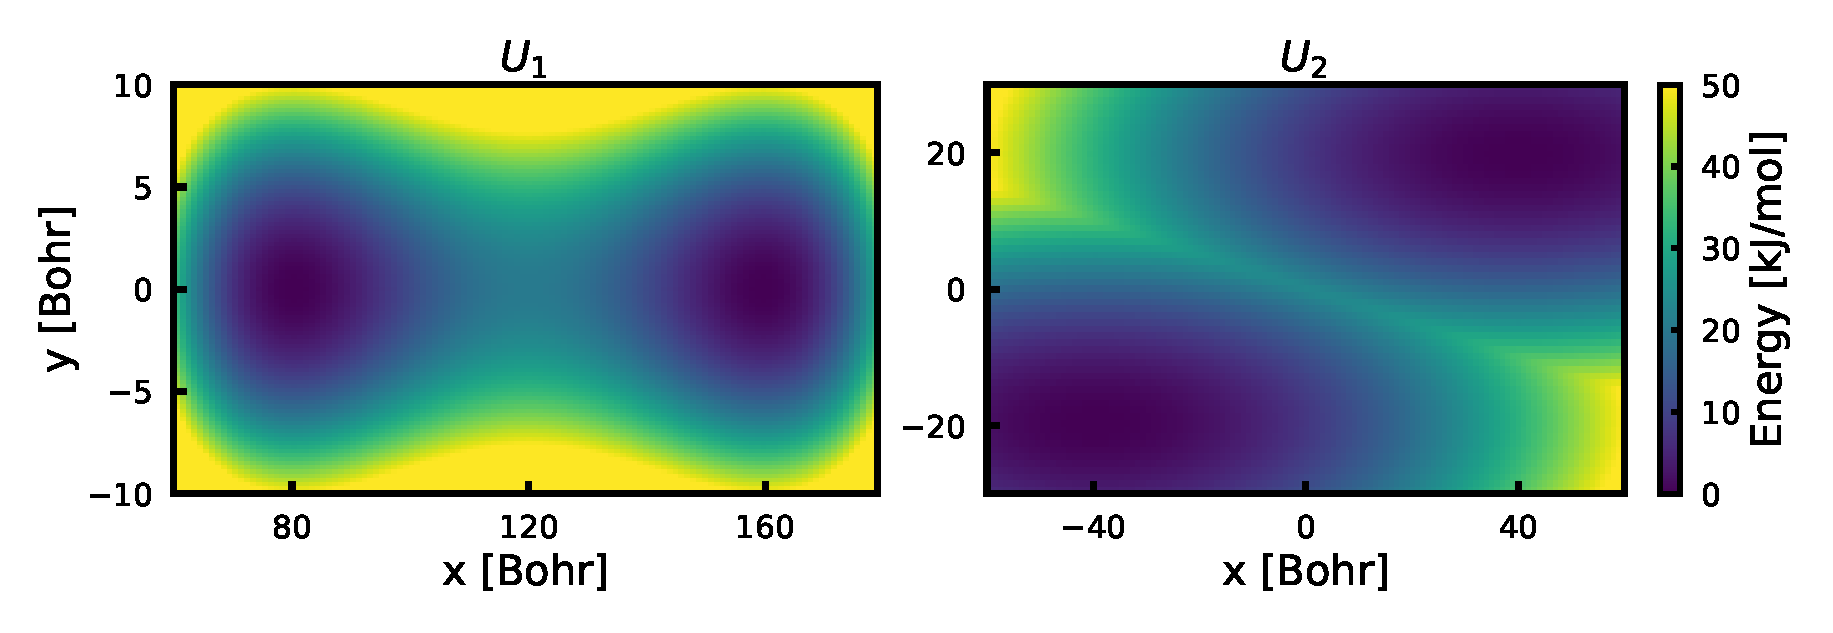
\includegraphics[width=1.0\textwidth]{bilder/U}
    \caption{Potentials for test calculations, Minima of $U_1$ are at located at (80,0) and (160,0). Minima of $U_2$ are located at (-40,-20) and (40,20). In both potentials minima are separated by free energy barriers of $20$~kJ/mol.}
\label{fig:potentials}%
\end{figure}
To simulate the particles dynamics a Velocity Verlet\autocite{swope1982computer} integrator is applied with a time step of 5~fs.
The initial momenta are drawn randomly from a Maxwell-Boltzmann distribution at 300~K.
Afterwards the temperature is controlled at 300~K by a Langevin thermostat\autocite{kroger2005models} with friction constant 0.001~fs$^{-1}$.
Crucial to the metastability of the system is the ratio of thermal energy~$k_B T$ to the barrier height.
Here, we always use transition barriers of height 8~$k_B T$ (20~kJ/mol).
Spontaneous transitions between minima in unbiased simulations can therefore be expected to be rare events.
All test simulation are completely performed in Python.

\section{Molecular Dynamics Simulations}
\label{sec:comp MD}
For QM simulations a Python interface for the in-house program suite FermiONs++\autocite{} was used.
Propagation of atomic coordinates with the Velocity Verlet\autocite{swope1982computer} integrator and temperature control with the Langevin thermostat\autocite{kroger2005models} (see algorithm~\ref{alg:ABM}) is done in Python.
For QM energy and gradient evaluation the PyFermiONsInterface was used.
All systems are simulated in vacuum.
To generate starting structures for MD simulations minimum energy geometries are obtained with the FermiONs intern geometry optimizer. MD simulations always consist of the following three steps:
\begin{enumerate}
  \item \textit{Heating}: Simulations are heated from 1~K to 300~K in 3000 time steps with a step size of 0.1~fs. Initial momenta are randomly drawn from a Maxwell-Boltzmann distribution. The velocities are rescaled every 10~time steps to increase the temperature by 1~K.
  \item \textit{Equillibration}: For thermal equilibration of the heated system is simulated for 1.0~ps under application of the Langevin thermostat at 300~K with a friction coefficient of 0.001~fs$^{-1}$. The time-step is increased to 0.5~fs. To produce starting structures for free energy estimation the system is also confined to the range of interest in CV space with harmonic walls.
  \item \textit{Production}: For production runs the equilibrated system is simulated under additional application of some enhanced sampling algorithm (see section~\ref{sec:comp ABM}).
\end{enumerate}

\section{Adaptive Biasing Implementation}
\label{sec:comp ABM}
All biasing algorithms are implemented in Python under extensive use of NumPy\autocite{harris2020array} and the PyFermiONsInterface.
For all methods the range of interest in CV space ($\xi_{min},\xi_{max}$), as well as the bin width $\Delta\xi$ are input parameters.
Simulations are restraint to this range by harmonic walls of the form
\begin{equation}
U^c(\xi) =\left\{\begin{array}{ll} \frac{k^c}{2}\bigl(\xi(\textbf{x}) - \xi^c_{min} \bigr)^2, & \xi \leq \xi^c_{min} \\
                                   \frac{k^c}{2}\bigl(\xi(\textbf{x}) - \xi^c_{max} \bigr)^2, & \xi \geq \xi^c_{max} \\
                                    0, & \text{otherwise}
          \end{array}\right.
\label{eq:harmonic wall}
\end{equation}
with restraining force constant $k^c$ and boundary of the simulation $\xi^c$.
For all simulations a stiff restraining force constant of $k^c=1000$~kJ/(mol$\Delta\xi^2$) is applied. The choice of boundaries ($\xi^c_{min}$,$\xi^c_{max}$) depends on the specific method and will be discussed in the following sections.
Probability distributions and free energy estimates are computed on fixed grids of the form ($f(\xi_{min}),f(\xi_{min}+\Delta\xi),...,f(\xi_{max})$).
All algorithms are computationally lightweight compared to QM energy and force evaluations and their impact on the overall computation time is negligible.

\subsection{MtD/WTM}
\label{subsec:implement MtD}
MtD/WTM potentials are accumulated on grids and free energy estimates obtained from equations~\ref{eq:F est MtD}/\ref{eq:F est WTM} are written to an output file in fixed intervals.
For MtD the height and variance of Gaussian hills $W$ and $\sigma_G$, as well as frequency of hill creation $\tau_G$ are input parameters. For WTM additionally $\Delta T$ is chosen to control how fast the Gaussian height decreases. Default parameters are given in table~\ref{tab:metaparams}.
\begin{table}[H]
      \centering
         \caption{Default parameters for MtD/WTM simulations.}
         \begin{tabular}{ c  c }
                 \hline
                  $\sigma_G$  & -        \\
                  $W$         & 1~kJ/mol \\
                  $\tau_G$    & 10~fs    \\
                  $\Delta T$  & 2000~K   \\
                 \hline
      \end{tabular}
      \label{tab:metaparams}
\end{table}
The MtD/WTM bias forces given by derivatives of eq.~\ref{eq:U_mtD}/\ref{eq:WTM} are also summed together and saved on a grid between update times of the potential.
In long simulations this is much more efficient than evaluating each hill at every step and yields negligible errors.\autocite{fiorin2013using}
The boundaries for the confinement of the simulation are set to
$\xi^c_{min}=\xi_{min}+2\Delta\xi$ and $\xi^c_{max}=\xi_{max}-2\Delta\xi$ for the lower and higher boundary, respectively, to avoid that the system is pushed out of the grid by the repulsive MtD/WTM potential.
To avoid that the bias forces suddenly vanish at the boundary they are calculated from hill centers near the margin, if the system still leafs the grid.
The resulting PMF will show a sharp increase at the margin, where the wall potential kicks in.

\subsection{ABF, eABF and WTM-eABF}
For ABF calculations two accumulators are used to store the biased histogram and sum of instantaneous force samples. The mean force is evaluated according to eq.~\ref{eq:mean force}.
The only ABF specific input parameter is the number of samples $N_{full}$ given to ramp function~\ref{eq:ramp}.
Force samples are calculated by eq.~\ref{eq:inst ABF force} and the inverse gradient is always chosen as $\textbf{v}_i = \nabla \xi_i/|\nabla \xi_i|^2$. Expressions for the divergence of $\textbf{v}_i$ for all applied CVs are given in the Appendix.
Constraints~\ref{eq:cond1} and \ref{eq:cond2} have to be fulfilled by choice of CV.
Harmonic walls are used to constrain the system to the range of interest.
Since the ABF force is not repulsive it is sufficient to apply the restraining force directly at the margin of the grid ($\xi^c_{min}=\xi_{min}$, $\xi^c_{max}=\xi_{max}$).

A flowchart of the full eABF/CZAR algorithm is given in figure~\ref{fig:eABF flowchart}.
The mass of the fictitious particle $m_\lambda$ and force constant $k_\lambda$ of its harmonic coupling to the physical system are free parameters.
Instead of directly choosing $k_\lambda$ the \textit{thermal width} of coupling $\sigma_\lambda$ is used as input parameter, which determines $k_\lambda$ by the following expression:
\begin{equation}
  k_\lambda = \frac{1}{\beta \sigma^2}
\end{equation}
The propagation of fictitious particles with a Velocity-Verlet\autocite{swope1982computer} integrator and temperature control by a Langevin thermostat\autocite{kroger2005models} is done completely independent of the physical system, but always using the same parameters.
$\xi$-conditioned expressions for CZAR are stored independently of $\lambda$-conditioned expressions for the eABF bias and CZAR estimates for the thermodynamic force on $\xi$ are computed at output times.
Additionally CZAR can be evaluated from trajectories of $\xi$ and $\lambda$ after the simulation has finished.
This way enhanced sampling and free energy estimation are completely independent.
MtD/WTM potentials and forces for (meta/WTM)-eABF are calculated as described in section~\ref{subsec:implement MtD} and eABF forces are accumulated separately.
Boundaries for the confinement of $\lambda$ are set to $\xi^c_{min}=\xi_{min}+2\sigma_\lambda$ and $\xi^c_{max}=\xi_{max}-2\sigma_\lambda$ for the lower and higher boundary, respectively. This way save confinement of $\xi$ to the region of interest is ensured only by its coupling to $\lambda$.

For 1D CVs PMFs are obtained at output times by numerically integrating the ABF or CZAR estimates of the thermodynamic force with the rectangular rule.\autocite{davis2007methods}
To generate 2D PMFs force estimates for both dimensions are stored and integrated separately with the FEM method.
For this purpose four control points are obtained between original data points by linear interpolation. The RMSD between B-spline functions and control points (eq. \ref{eq:RMSD}) is than minimized with the Broyden–Fletcher–Goldfarb–Shanno (BFGS) algorithm.\autocite{nocedal2006numerical}

\begin{figure}[H]
   \caption{
     Flowchart of the eABF algorithm. $k_{\lambda}$ and $k_\xi$ denote $\lambda$ or $\xi$ conditioned bin indices, respectively, in bins with size $\Delta\xi$. $P^B_\lambda$ and $P^B_\xi$ are $\lambda$- or $\xi$- conditioned histograms and $R$ is the ABF ramp function. $F_B$ is the sum of force samples. Outputs are written in fixed intervals.
   }

        \centering
        \begin{tikzpicture}[minimum size=5mm,node distance=4cm and 7cm,>=stealth,bend angle=45,auto]
        \node [block] (xi) {$\xi \leftarrow f(\textbf{x})$};
        \node [block, below of=xi] (langevin) {Langevin dynamics of extended system};
        \node [block, below of=langevin,yshift=-0.5cm] (F_ext) {add harmonic force of extended system to QM/MM forces};

        \node [decision, below of=F_ext, yshift=-1cm] (decide_lambda) {$\xi_{min}\leq \lambda \leq \xi_{max}$};

        \node [block, below of=decide_lambda,xshift=-3cm] (la_bin) {$k_\lambda = \lfloor \frac{|\lambda - \xi_{min}|}{\Delta \xi} \rfloor$};
        \node [block, below of=la_bin] (la_hist) {$P^B_\lambda(k_\lambda) \pluseqq 1$};
        \node [block, below of=la_hist] (R) {$R(k_\lambda) = f(k_\lambda)$ (eq. \ref{eq:ramp})};
        \node [block, below of=R] (F_B1) {$\overline{F}_B(k_\lambda)=\frac{(\lambda_i-\braket{\xi_i}_{\lambda_i})}{\sigma_i^2}$};
        \node [block, below of=F_B1] (F_B2) {$\textbf{F}(\textbf{x},\lambda) \pluseqq R(k_\lambda)\overline{F}_B(k_\lambda)\nabla\lambda$};

      %  \node [block, right of=R,xshift=4cm] (conf1) {confine $\lambda$ to range of interest};

        \node [decision, below of=F_B2,xshift=3cm] (decide_xi) {$\xi_{min}\leq \xi \leq \xi_{max}$};

        \node [block, below of=decide_xi,xshift=-3cm] (xi_bin) {$k_\xi = \lfloor \frac{|\xi - \xi_{min}|}{\Delta \xi} \rfloor$};
        \node [block, below of=xi_bin] (xi_hist) {$P^B_\xi(k_\xi) \pluseqq 1$};
        \node [block, below of=xi_hist] (F_corr) {$\overline{F}_{corr}(k_\xi)=\frac{(\braket{\lambda_i}_{\xi_i}-\xi_{i})}{\sigma_i^2}$};

      %  \node [block, right of=xi_hist,xshift=4cm] (conf2) {confine $\xi$ to range of interest};

        \node [block,below of=F_corr,xshift=3cm,yshift=-0.5cm] (MD1) {Finish Langevin dynamics of extended system};

        \node [decision, left of=decide_xi,xshift=-5.5cm] (output) {write output?};
        \node [block, left of=F_B1,xshift=-6cm] (CZAR) {calculate CZAR according to eq. \ref{eq:CZAR}};
        \node [block, left of=la_bin,xshift=-6cm] (out) {write output};

        \node [block, above of=output,yshift=10cm] (MD2) {MD step of physical system. (compare Algorithm \ref{alg:ABM})};

        \path [line] (xi) -- (langevin);
        \path [line] (langevin) -- (F_ext);
        \path [line] (F_ext) -- (decide_lambda);

        \path [line] (decide_lambda) -- node [above,xshift=-0.3cm] {yes} (la_bin);
        \path [line] (la_bin) -- (la_hist);
        \path [line] (la_hist) -- (R);
        \path [line] (R) -- (F_B1);
        \path [line] (F_B1) -- (F_B2);

        \draw [->] (decide_lambda) -- node {no} (decide_xi);

        \path [line] (F_B2) -- (decide_xi);
      %  \path [line] (conf1) -- (decide_xi);

        \draw [->] (decide_xi) -- node [above,xshift=-0.3cm] {yes} (xi_bin);
        \path [line] (xi_bin) -- (xi_hist);
        \path [line] (xi_hist) -- (F_corr);

%\draw [->] (decide_xi) -- node {no} (conf2);

        \path [line] (F_corr) -- (MD1);
        \path [line] (decide_xi) -- node [right] {no} (MD1);

        \path [line] (MD1) -| (output);
        \path [line] (output) -- node [below,yshift=-0.2cm] {yes} (CZAR);
        \path [line] (CZAR) -- (out);
        \path [line] (out) -- (MD2);

        \draw[->] (output) -- node [right] {no} (MD2);
        \draw[->] (MD2) |- (xi);

        \end{tikzpicture}
        \label{fig:eABF flowchart}
\end{figure}

	\chapter{Results and Discussion}
\label{cha:results}

\section{Convergence}

  \chapter{Appendix}
\label{cha:appendix}

\section{Definition of Collective Variables}
\label{sec:reaction coordinates}

In the present work distances, projected distances, angles and torsion angles between groups of atoms were used as collective variables for Umbrella Sampling, metaD, ABF, eABF or meta-eABF simulations.
Below analytic expressions for the calculation of all CVs, their gradients, inverse gradients and divergence of inverse gradients are given.

The center of mass $r^C$ of a group of $N$ atoms is calculated according to
\begin{equation}
  r^C(\textbf{x}) = \frac{1}{M^C} \sum_{i=0}^N m_i r_i
\end{equation}
with mass of each atom $m_i$ and Cartesian coordinates $r_i = (x_i,y_i,z_i)$. $M^C$ is the mass of the group.
All following collective variables are calculated between centers of mass. The index C will be dropped for convenience.
To obtain derivatives of single atoms the gradient its corresponding group is weighted with $m_i/M$.
The distances between group i and j is given by
\begin{equation}
 r_{ij} = r_j - r_i
\end{equation}
and the absolute distance is $d_{ij} = \| r_{ij}\|$.
The derivatives with respect to $r_i$ and $r_j$ are defined by
\begin{equation}
  \frac{\partial d_{ij}}{\partial r_j} = \frac{r_{ij}}{\|r_{ij}\|} = \hat{r}_{ij}
\end{equation}
\begin{equation}
  \frac{\partial d_{ij}}{\partial r_i} = - \hat{r}_{ij}
\end{equation}
where the hat denotes unit vectors.
The projection of distance $\| r_{ij}\|$ onto another axis $r_{jk}$ is defined by
\begin{equation}
  d^p_{ij} = r_{ij} \cdot \hat{r}_{jk}
\end{equation}
and the derivative of the projection is defined by
\begin{equation}
   \frac{\partial d^p_{ij}}{\partial r_i} = -\hat{r}_{jk}
\end{equation}
\begin{equation}
   \frac{\partial d^p_{ij}}{\partial r_j} = \hat{r}_{jk}
\end{equation}
The bond angle $\theta$ between three centers ($r_i, r_j, r_k$) is defined by the dot product of bond distances $r_{ji}$ and $r_{jk}$:
\begin{equation}
  \cos \theta = \hat{r}_{ji} \cdot \hat{r}_{jk}
\end{equation}
The gradient of $\theta$ is then given by
\begin{equation}
  \frac{\partial \theta}{\partial r_i} = \frac{(r_{ji} \times (r_{ji} \times r_{jk})) }{\| r_{ij}\| \| (r_{ji} \times (r_{ji} \times r_{jk})) \|}
\end{equation}
\begin{equation}
  \frac{\partial \theta}{\partial r_k} = \frac{\| (r_{kj} \times (r_{ji} \times r_{ji})) \|}{\| r_{kj}\| \| (r_{kj} \times (r_{ji} \times r_{ji})) \|}
\end{equation}
\begin{equation}
  \frac{\partial \theta}{\partial r_j}= -\frac{\partial \theta}{\partial r_i} - \frac{\partial \theta}{\partial r_k}
\end{equation}
The torsion angle $\phi$ between four Cartesian coordinates ($r_i, r_j, r_k, r_l$) is given by:
\begin{equation}
  \tan \phi = \frac{(\hat{r}_{ij} \times n_1) \cdot n_2}{n_1 \cdot n_2}
\end{equation}
with
\begin{equation}
  n_1 = r_{jk} - (r_{ij} \cdot \hat{r}_{jk})\hat{r}_{jk}
\end{equation}
\begin{equation}
  n_2 = r_{kl} - (r_{kl} \cdot \hat{r}_{jk})\hat{r}_{jk}
\end{equation}
The derivative of $\phi$ in Cartesian coordinates is given by:
\begin{equation}
  \frac{\partial\phi}{\partial r_i} = - \frac{\hat{r}_{ji}\times\hat{r}_{jk}}{\|r_{ij}\|\sin^2\theta_{ijk}}
\end{equation}
\begin{equation}
  \frac{\partial\phi}{\partial r_l} = - \frac{\hat{r}_{kl}\times\hat{r}_{jk}}{\|r_{kl}\|\sin^2\theta_{jkl}}
\end{equation}
\begin{equation}
  \frac{\partial\phi}{\partial r_j} = c_{ijk}\frac{\partial\phi}{\partial r_i} - b_{lkj}\frac{\partial\phi}{\partial r_l}
\end{equation}
\begin{equation}
  \frac{\partial\phi}{\partial r_k} = - \frac{\partial\phi}{\partial r_i} - \frac{\partial\phi}{\partial r_l} - \frac{\partial\phi}{\partial r_j}
\end{equation}
with
\begin{equation}
  c_{ijk} = \frac{\|r_{ij} \| \cos\theta_{ijk}}{\|r_{jk} \|}-1
\end{equation}
\begin{equation}
  b_{lkj} = \frac{\|r_{kl} \| \cos\theta_{jkl}}{\|r_{jk} \|}
\end{equation}
where $\partial \phi/\partial r_j$ and $\partial \phi/\partial r_k$ are defined in such a way, that the sum of torques and derivatives is zero.

Always choosing as inverse gradient $\textbf{v}(\xi) = \nabla \xi/\|\nabla \xi \| ^2$ the divergence of vector fields $\textbf{v}_i(\xi)$ are given by
\begin{equation}
  \nabla \cdot \textbf{v}(d) = \frac{2}{d},
\end{equation}
\begin{equation}
  \nabla \cdot \textbf{v}(d^p) = 0,
\end{equation}
\begin{equation}
  \nabla \cdot \textbf{v}(\theta) = \cot \theta,
\end{equation}
\begin{equation}
  \nabla \cdot \textbf{v}(\phi) = 0,
\end{equation}
for distances, projected distances, angles and dihedrals, respectively.

	\appendix                     % Anhang

	\backmatter
	\pagenumbering{Roman}                    % für letzte Verzeichnisse wieder romanische Nummerierung
	\sectionnumbering{Roman}
	\setcounter{page}{\theromanPagenumber}   % setzt die aktuelle Seitenzahl von vorne für die romanische Nummerierung fest

	\listoftables
	\listoffigures

%   \nocite{*}								 % auch Quellen die nicht verwendet wurden tauchen in Literaturverzeichnis auf
	\inputencoding{utf8}
	\printbibliography[title=Bibliography]   % gibt Literaturverzeichnis aus

\end{document}
